\documentclass[12pt]{article}
\usepackage{float}
\usepackage{placeins}
\usepackage{sbc-template}
\usepackage{graphicx,url}
\usepackage[brazil]{babel}
\floatplacement{figure}{H}
\floatplacement{table}{H}
\usepackage[utf8]{inputenc}
\usepackage{booktabs}
\usepackage[table]{xcolor}
\usepackage[activate={true,nocompatibility},final,tracking=true,kerning=true,spacing=true]{microtype}

\sloppy

\title{HormuzNet: Monitoramento Marítimo Descentralizado e Resiliência em Sistemas Críticos}

\author{Luis Felipe Pereira de Carvalho\inst{1}}

\address{Departamento de Tecnologia -- Universidade Estadual de Feira de Santana (UEFS)\\
  44036-900 -- Feira de Santana -- Bahia
  \email{luisoftbr@outlook.com.br}}

\begin{document}

\maketitle

\begin{abstract}
[Context] Maritime monitoring of strategic routes demands distributed architectures
capable of integrating heterogeneous sensors with high availability and no single
point of failure. [Problem] Centralized architectures introduce a critical single
point of failure: if the central server becomes inoperative, the entire monitoring
and maritime rescue infrastructure is immediately disrupted. [Contribution] This
work presents HormuzNet, a decentralized maritime monitoring system for the Strait
of Hormuz that replaces the centralized model with an autonomous cooperative mesh
of brokers, using Lamport's Logical Clocks for global event ordering and distributed
mutual exclusion. [Methodology] The system was implemented in Go using native UDP
Multicast for redundant telemetry, persistent TCP with fallback logic for drone
coordination, and WebSocket for real-time tactical visualization. The infrastructure
was validated in a containerized environment with 34 Docker containers distributed
across two physical hosts. [Results] The architecture demonstrated effective
elimination of single points of failure, automatic broker recovery, consistent
mission dispatching with an average latency under 1.5 seconds, and correct Lamport
clock synchronization under simultaneous load from 18 sensors.
\end{abstract}

\begin{resumo}
\sloppy
[Contexto] O monitoramento marítimo de rotas estratégicas exige arquiteturas
distribuídas capazes de integrar sensores heterogêneos com alta disponibilidade
e ausência de pontos únicos de falha. [Problema] Arquiteturas centralizadas
introduzem um ponto único de falha crítico: se o servidor central torna-se
inoperante, toda a infraestrutura de monitoramento e salvamento marítimo é
imediatamente interrompida. [Contribuição] Este trabalho apresenta o HormuzNet,
um sistema descentralizado de monitoramento marítimo para o Estreito de Ormuz que
substitui o modelo centralizado por uma malha cooperativa autônoma de \textit{brokers},
utilizando Relógios Lógicos de Lamport para ordenação global de eventos e exclusão
mútua distribuída. [Metodologia] O sistema foi implementado em Go com UDP
\textit{Multicast} nativo para telemetria redundante, TCP persistente com lógica de
\textit{fallback} para coordenação de drones e WebSocket para visualização tática
em tempo real. A infraestrutura foi validada em ambiente conteinerizado com 34
contêineres Docker distribuídos em duas máquinas físicas. [Resultados] A arquitetura
demonstrou eliminação efetiva de pontos únicos de falha, recuperação automática de
\textit{brokers}, despacho consistente de missões com latência média inferior a 1,5
segundos e sincronização correta dos relógios de Lamport mesmo sob carga
simultânea de 18 sensores.
\end{resumo}

\section{Introdução}
\label{sec:introducao}
O monitoramento de infraestruturas críticas, como o Estreito de Ormuz, constitui um desafio complexo no campo dos sistemas distribuídos. O estreito é uma das rotas marítimas mais estratégicas do mundo, responsável por aproximadamente 20\% do tráfego global de petróleo \cite{tanenbaum2021redes}. A necessidade de rastrear continuamente embarcações, detectar anomalias ambientais e despachar recursos de resposta a emergências exige uma arquitetura de software robusta, de alta disponibilidade e capaz de operar mesmo diante de falhas parciais na infraestrutura.

Sistemas baseados em modelo de \textit{broker} centralizado, como o FarmNode desenvolvido no projeto anterior, introduzem um ponto único de falha (\textit{Single Point of Failure} -- SPOF) crítico: se o servidor central torna-se inoperante, toda a infraestrutura de monitoramento e salvamento marítimo é interrompida imediatamente. Adicionalmente, a alocação concorrente de recursos escassos --- como drones de patrulhamento disputados por múltiplas ocorrências simultâneas --- pode resultar em inanição de tarefas ou impasse (\textit{deadlock}) distribuído.

Para mitigar esses problemas, este trabalho apresenta o \textbf{HormuzNet}, um sistema de monitoramento marítimo descentralizado baseado em uma malha cooperativa de \textit{brokers}. O HormuzNet elimina SPOFs ao distribuir o processamento por meio de uma arquitetura híbrida que combina o modelo cliente-servidor em dois níveis com uma malha ponto a ponto (P2P). A consistência de dados e a ordenação global de eventos são garantidas pelos Relógios Lógicos de Lamport \cite{lamport1978time}, enquanto a exclusão mútua distribuída resolve a concorrência pelo despacho de drones.

O sistema foi implementado em Go com protocolos nativos de rede: UDP/IP Multicast para telemetria redundante, TCP/IP persistente com lógica de \textit{fallback} para coordenação de drones autônomos, e WebSocket para visualização tática em tempo real. A infraestrutura foi validada com 34 contêineres Docker distribuídos entre duas máquinas físicas interconectadas por rede LAN Gigabit.

Os resultados demonstram que a malha de \textit{brokers} reage autonomamente a falhas por meio de \textit{Ring Failover} e eleição Bully, realizando o despacho de drones com latência média inferior a 1,5\,s e sem inconsistências nas filas de prioridade distribuídas.


\section{Fundamentação Teórica}
\label{sec:fundamentos}
A resiliência do HormuzNet apoia-se em quatro pilares teóricos: arquitetura distribuída descentralizada, protocolos de rede em camadas, concorrência gerenciada e algoritmos de coordenação lógica.

\subsection{Arquiteturas Distribuídas e Modelos de Comunicação}

Sistemas distribuídos organizam nós autônomos que cooperam por troca de mensagens \cite{tanenbaum2021redes}. O modelo cliente-servidor tradicional centraliza o processamento em um único ponto, o que introduz pontos únicos de falha e gargalos de desempenho; a descentralização P2P distribui responsabilidades entre os nós para obter maior tolerância a falhas e redundância \cite{tanenbaum2021redes}. O HormuzNet combina os dois modelos: sensores e drones operam como clientes dos \textit{brokers} de setor (camada 1), enquanto os \textit{brokers} formam entre si uma malha P2P cooperativa (camada 2).

Os protocolos de rede foram selecionados com base no \textit{trade-off} entre confiabilidade e latência. O UDP (RFC~768 \cite{rfc768}) sobre IP (RFC~791 \cite{rfc791}) oferece entrega sem conexão e baixo \textit{overhead}, adequado para telemetria redundante via \textit{Multicast} (RFC~1112 \cite{rfc1112}), em que a perda eventual de um datagrama é tolerável diante do fluxo contínuo dos sensores. O TCP (RFC~793 \cite{rfc793}) fornece canal bidirecional confiável e com entrega ordenada, indispensável para mensagens de coordenação da malha (\textit{gossip}, Lamport, Bully) e comandos de despacho de drones. O WebSocket (RFC~6455 \cite{rfc6455}) acrescenta comunicação \textit{full-duplex} em tempo real sobre TCP, permitindo que o monitor tático receba atualizações instantâneas sem a necessidade de \textit{polling} HTTP.

\subsection{Concorrência em Go e Estruturas de Dados Distribuídas}

A linguagem Go implementa o modelo CSP (\textit{Communicating Sequential Processes}) \cite{donovan2015go}: \textit{goroutines} são \textit{threads} leves gerenciadas em espaço de usuário, enquanto canais proveem comunicação segura entre elas. Para acesso direto à memória compartilhada, \textit{mutexes} refinados por recurso (\texttt{dronesMu}, \texttt{ocorrenciasMu}) protegem regiões críticas sem introduzir gargalos globais. Filas de prioridade baseadas em \textit{heap} binário garantem que ocorrências críticas sejam atendidas primeiro; o algoritmo de \textit{aging} previne inanição ao incrementar gradualmente a prioridade de elementos que aguardam há muito tempo na fila.

\subsection{Relógio Lógico de Lamport e Algoritmo Bully}

Lamport \cite{lamport1978time} propôs \textit{timestamps} lógicos para ordenação total de eventos em sistemas distribuídos sem relógio físico global: cada processo mantém um contador inteiro incrementado a cada evento local e atualizado ao receber mensagens externas, preservando a relação de causalidade entre eventos. No HormuzNet, o relógio de Lamport é sincronizado a cada mensagem trocada na malha P2P, garantindo que ocorrências inseridas concorrentemente em \textit{brokers} distintos sejam ordenadas de forma global e determinística.

Para a eleição do \textit{broker} líder, utiliza-se o Algoritmo Bully \cite{tanenbaum2021redes}: ao detectar a ausência de \textit{heartbeat} do coordenador, um nó envia \texttt{ELEICAO} a todos os \textit{brokers} com identificador superior; o nó de maior ID que responder torna-se o novo líder e anuncia sua posição à malha, garantindo convergência rápida mesmo em cenários de falha em cascata.

\subsection{Docker e Emulação Distribuída}

A tecnologia de contêineres Docker isola processos compartilhando o \textit{kernel} do sistema hospedeiro, proporcionando portabilidade e consistência de ambiente entre máquinas distintas. O Docker Compose permite definir topologias de múltiplos contêineres e suas redes virtuais em um único arquivo declarativo. No HormuzNet, essa tecnologia foi empregada para emular a topologia distribuída com 34 contêineres independentes em máquinas rodando Linux Ubuntu e Linux Mint.


\section{Metodologia}
\label{sec:metodologia}
Esta seção descreve os materiais, métodos e decisões de projeto adotados no desenvolvimento do HormuzNet. São detalhados a arquitetura do sistema, os protocolos de comunicação implementados, os algoritmos distribuídos de tolerância a falhas e o ambiente de emulação utilizado para validação.

\subsection{Material e Método}
\label{sub:material_metodo}

O desenvolvimento e a avaliação experimental do HormuzNet basearam-se em computadores conectados via rede física Gigabit Ethernet no Laboratório LARSID da Universidade Estadual de Feira de Santana (UEFS). Os hosts executaram distribuições Linux (\textbf{Ubuntu} e \textbf{Mint}). O ambiente de software compreendeu:
\begin{itemize}
    \item \textbf{Linguagem de Programação:} Go (versão 1.21.2);
    \item \textbf{Motor de Contêineres:} Docker (versão 24.0.5);
    \item \textbf{Orquestrador:} Docker Compose (versão 2.20.2).
\end{itemize}

Foram testadas duas topologias: a \textbf{local}, com todos os contêineres em um único \textit{host} compartilhando rede virtual \textit{bridge}, e a \textbf{distribuída}, com a infraestrutura dividida entre duas máquinas físicas via LAN Gigabit. O cenário padrão instanciou \textbf{34 contêineres}: 9 \textit{brokers} (B1--B9), 6 drones autônomos, 18 sensores inteligentes (2 por setor) e 1 monitor tático. As métricas foram coletadas via chamadas \textit{curl} ao endpoint \texttt{/api/estado}, logs em tempo real pelo script \texttt{terminais.sh} e saída do comando \texttt{docker stats}.

\subsection{Arquitetura do Sistema}
\label{sub:arquitetura}

O HormuzNet afasta-se do modelo hierárquico centralizado do FarmNode, que dependia de um único \textit{broker} como SPOF. Em vez disso, adota um modelo \textbf{cliente-servidor em dois níveis}:
\begin{enumerate}
    \item[(i)] No primeiro nível, sensores e drones comportam-se como clientes dos \textit{brokers} de setor (servidores locais);
    \item[(ii)] No segundo nível, os \textit{brokers} formam entre si uma malha descentralizada P2P cooperativa.
\end{enumerate}

Essa topologia híbrida garante que mensagens de telemetria e coordenação circulem de forma redundante e resiliente pela malha geográfica. A Figura~\ref{fig:arquitetura} apresenta a organização dos componentes e a dinâmica de auto-organização da malha.

\begin{figure}[ht]
  \centering
  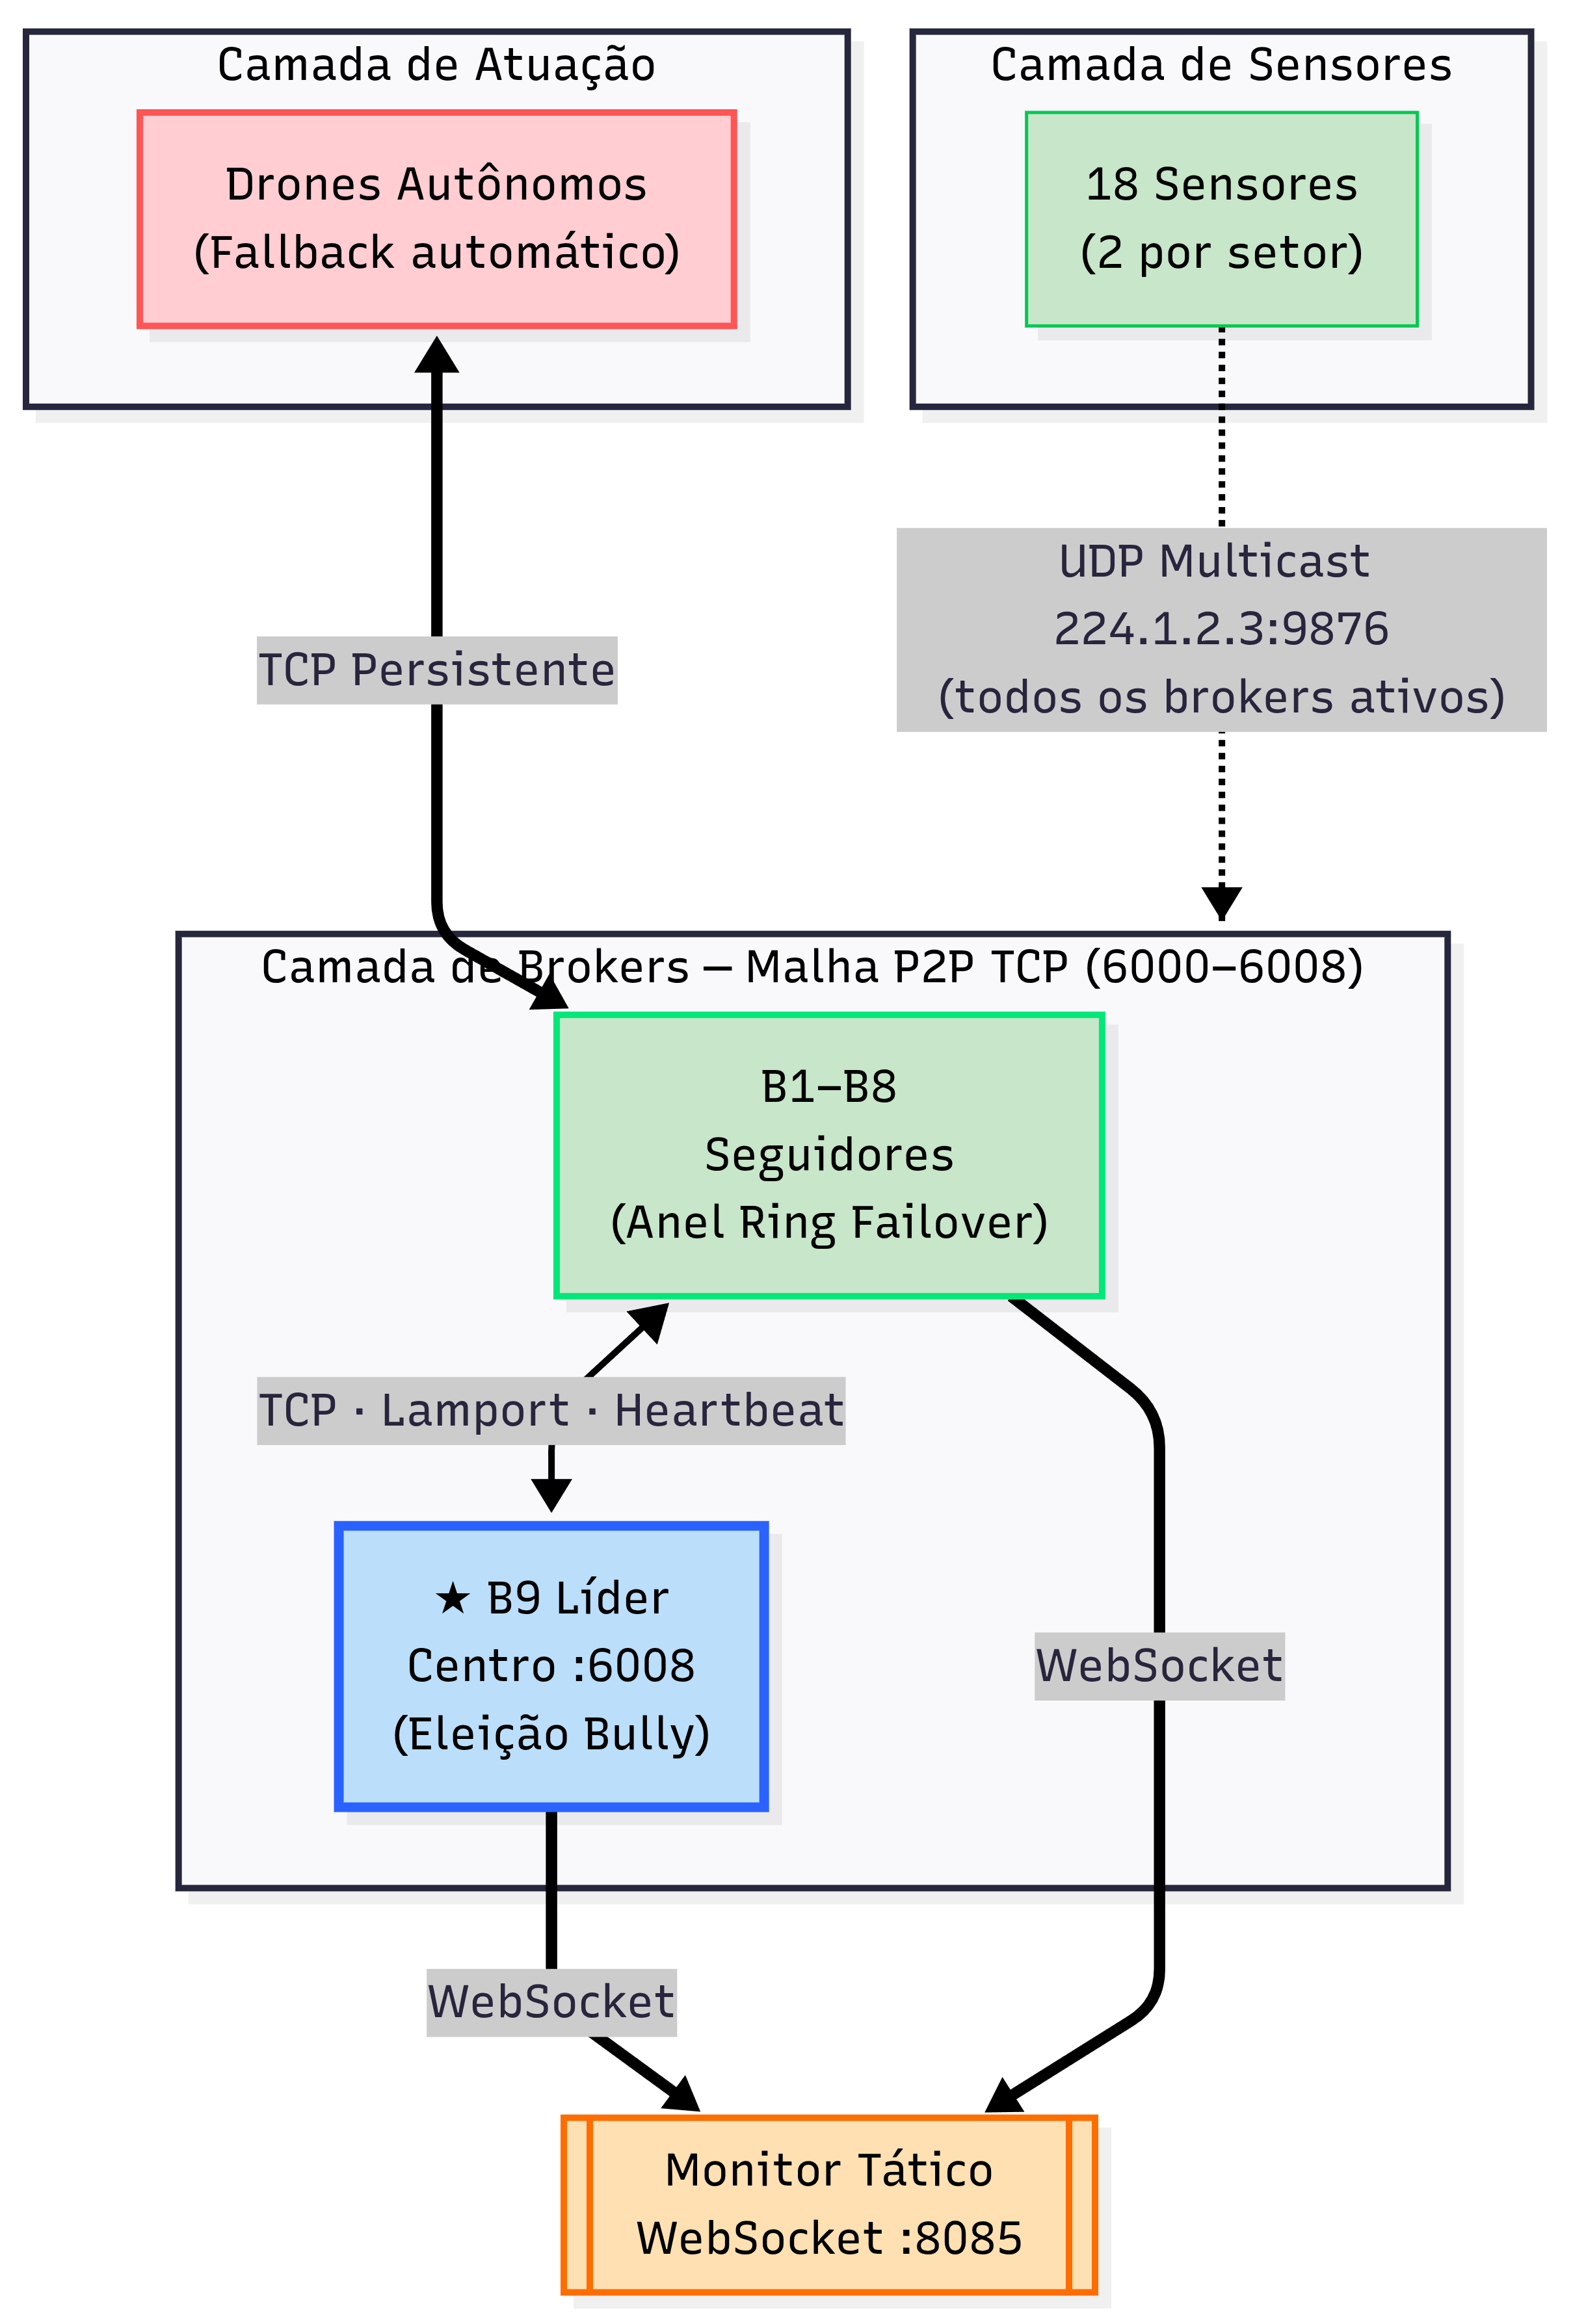
\includegraphics[width=0.45\textwidth]{figuras/arquitetura.png}
  \caption{Arquitetura descentralizada do HormuzNet com camadas de sensores, \textit{brokers} e drones. Fonte: Próprio Autor.}
  \label{fig:arquitetura}
\end{figure}

\subsection{Protocolo de Comunicação}
\label{sub:protocolo}

A troca de informações ocorre por meio de canais específicos detalhados na Tabela~\ref{tab:protocolo}.

\begin{table}[ht]
  \centering
  \sloppy
  \caption{Portas, protocolos e formatos dos canais de comunicação do HormuzNet. Fonte: Próprio Autor.}
  \label{tab:protocolo}
  \begin{tabular}{p{2.6cm}p{2.4cm}p{1.6cm}p{1.8cm}p{3.0cm}}
    \toprule
    \textbf{Fluxo} & \textbf{Protocolo} & \textbf{Porta} & \textbf{Formato} & \textbf{Propósito} \\
    \midrule
    Sensor $\to$ Broker & UDP/IP Multicast & 9876 & JSON UTF-8 & Telemetria e alertas \\
    Broker $\leftrightarrow$ Broker & TCP/IP P2P & 6000--6008 & JSON/linha & \textit{Gossip}, Lamport, Bully \\
    Drone $\leftrightarrow$ Broker & TCP/IP & 6000--6008 & JSON/linha & Registro e despacho \\
    Broker $\to$ Monitor & TCP/IP & 6000--6008 & JSON/linha & Logs e descoberta \\
    Monitor $\to$ Dashboard & WebSocket & 8085 & JSON \textit{frame} & \textit{Snapshot} tático \\
    \bottomrule
  \end{tabular}
\end{table}

Na telemetria, sensores publicam datagramas JSON no grupo \textit{multicast} \texttt{224.1.2.3:9876}; a delimitação de mensagem é o próprio tamanho do datagrama UDP/IP \cite{rfc768,rfc791}. Nos fluxos TCP/IP de coordenação, cada mensagem JSON é terminada por \texttt{\textbackslash{}n} e lida via \texttt{bufio.Scanner}.

\subsection{Descoberta, Filas e Concorrência}
\label{sub:descoberta_filas}

Ao iniciar, cada \textit{broker} seguidor conecta-se ao líder e recebe a lista de membros ativos (\texttt{PEER\_LIST}), estabelecendo suas conexões TCP P2P dinamicamente. Drones registram-se no \textit{broker} de seu setor e, em caso de falha deste, executam \textit{fallback} automático para o vizinho seguinte na lista de setores. Cada \textit{broker} mantém um \textit{heap} binário \textit{thread-safe} com capacidade para até 262.144 ocorrências; o despacho seleciona o drone disponível de menor distância cartesiana ao incidente, emite o comando \texttt{DESPACHAR\_DRONE} via TCP e propaga a remoção do evento por \textit{broadcast} à malha. A concorrência é gerenciada com \textit{goroutines} por \textit{socket} e \textit{mutexes} por recurso, com \textit{timeout} de escrita de 2\,s para prevenir bloqueios.

\subsection{Confiabilidade: \textit{Heartbeat} e \textit{Ring Failover}}
\label{sub:confiabilidade}

\textit{Brokers} emitem \textit{heartbeats} a cada 5\,s para seus vizinhos P2P. Após 15\,s sem resposta, o nó é marcado como inativo: o vizinho anterior no anel lógico assume o setor (\textit{Ring Failover}), os drones do \textit{broker} inativo reconectam-se por \textit{backoff} ao próximo vizinho disponível e, caso o líder tenha falhado, os seguidores iniciam imediatamente o algoritmo Bully para eleição de novo coordenador.

\subsection{Emulação e Testes}
\label{sub:emulacao}

O ambiente de emulação injeta distúrbios realísticos de forma contínua: ocorrências permanecem na fila sob \textit{aging} de 30\,s, com incremento de criticidade a cada ciclo sem atendimento; drones em patrulha entram em alerta de ociosidade após 60\,s sem missão; e cada drone possui 10\% de probabilidade de ser abatido em trânsito, forçando o \textit{broker} a registrar a perda e re-enfileirar a ocorrência na malha.


\section{Resultados}
\label{sec:resultados}
A avaliação prática da arquitetura proposta sob condições de falha e estresse fornece evidências sobre sua viabilidade e eficiência. Esta seção apresenta os resultados funcionais e de desempenho obtidos e estabelece um comparativo com a arquitetura do FarmNode.

\subsection{Ambiente de Avaliação}
\label{sub:ambiente_avaliacao}

A validação experimental ocorreu por meio de cenários simulados de estresse e injeção de falhas no ambiente de contêineres descrito na Metodologia. A malha foi instanciada com 9 \textit{brokers}, 6 drones autônomos e 18 sensores georreferenciados. A avaliação distribuída envolveu a partição física do processamento entre duas máquinas interconectadas via LAN Gigabit no laboratório LARSID/UEFS, permitindo avaliar a latência de \textit{gossip} e o comportamento de sincronização sob rede física real.

\subsection{Resultados Funcionais}
\label{sub:resultados_funcionais}

Os testes de comportamento funcional validaram as rotinas de \textit{failover}, eleição de líder e redundância de recepção de telemetria. A Tabela~\ref{tab:resiliencia} sumariza os principais cenários testados e as respostas correspondentes do sistema.

\begin{table}[ht]
  \centering
  \sloppy
  \caption{Resultados funcionais do sistema diante de falhas injetadas. Fonte: Próprio Autor.}
  \label{tab:resiliencia}
  \begin{tabular}{p{0.8cm}p{4.2cm}p{6.0cm}p{1.0cm}}
    \toprule
    \textbf{ID} & \textbf{Cenário de Falha} & \textbf{Resposta do Sistema} & \textbf{Status} \\
    \midrule
    TR-01 & Queda do \textit{Broker} B3 (Nordeste) & B2 assume o Setor Nordeste via \textit{Ring Failover}; drones executam \textit{fallback} & OK \\
    TR-02 & Emissão de Alerta \textit{Multicast} & Recebido de forma redundante por todos os \textit{brokers} ativos & OK \\
    TR-03 & Drone Abatido em Missão & \textit{Broker} detecta perda de \textit{socket} TCP, remove drone e re-enfileira ocorrência & OK \\
    TR-04 & Conflito de \textit{Timestamps} & \textit{Brokers} ordenam ocorrências por prioridade e \textit{timestamp} de Lamport & OK \\
    TR-05 & Queda do Líder B9 (Centro) & Seguidores detectam ausência de \textit{heartbeat} e realizam eleição Bully & OK \\
    \bottomrule
  \end{tabular}
\end{table}

\subsection{Testes Automatizados}
\label{sub:testes_automatizados}

Testes unitários validaram a ordenação e o \textit{aging} do \textit{heap} de prioridades com inserção concorrente de chaves duplicadas. Testes de integração verificaram o \textit{pipeline} de serialização JSON em \textit{sockets} TCP/IP e a consistência dos relógios de Lamport sob carga massiva de \textit{goroutines}.

\subsection{Carga e Desempenho}
\label{sub:carga_desempenho}

As métricas de latência e consumo de recursos foram coletadas durante uma sessão de estresse de 10 minutos, com geração de alertas na taxa de 1 evento a cada 2 segundos por sensor. A Tabela~\ref{tab:performance} consolida os resultados quantitativos observados.

\begin{table}[ht]
  \centering
  \sloppy
  \caption{Métricas de desempenho obtidas em teste de estresse contínuo. Fonte: Próprio Autor.}
  \label{tab:performance}
  \begin{tabular}{p{5.5cm}p{2.5cm}p{5.0cm}}
    \toprule
    \textbf{Métrica} & \textbf{Valor} & \textbf{Observação} \\
    \midrule
    Tempo de despacho médio (s) & 1,5 & Da ocorrência ao despacho do drone \\
    Divergência de relógios de Lamport (ms) & 0 & Filas idênticas entre \textit{brokers} \\
    Uso médio de CPU por \textit{broker} (\%) & $<$ 5\% & Concorrência via \textit{goroutines} \\
    Uso médio de RAM por \textit{broker} (MB) & 12 & Inclui \textit{overhead} do \textit{heap} binário \\
    Taxa de sucesso de missões (\%) & $\approx$\,90\% & Taxa fixa de 10\% de abates simulados \\
    Latência de comunicação P2P (ms) & $<$ 10 & Média nas conexões da malha TCP/IP \\
    \bottomrule
  \end{tabular}
\end{table}

\subsection{Comparação com FarmNode}
\label{sub:comparacao_farmnode}

A Tabela~\ref{tab:comparacao} estabelece uma comparação estrutural e funcional direta entre o FarmNode e o HormuzNet, evidenciando os avanços de robustez obtidos.

\begin{table}[ht]
  \centering
  \sloppy
  \caption{Comparação entre FarmNode (centralizado) e HormuzNet (descentralizado). Fonte: Próprio Autor.}
  \label{tab:comparacao}
  \begin{tabular}{p{3.8cm}p{4.8cm}p{4.8cm}}
    \toprule
    \textbf{Critério} & \textbf{FarmNode (P1)} & \textbf{HormuzNet (P2)} \\
    \midrule
    Topologia & \textit{Broker} único centralizado & Malha de N \textit{brokers} \\
    Ponto único de falha & Existe & Eliminado (\textit{fallback} + \textit{heartbeat}) \\
    Coordenação de recursos & Implícita (1 servidor decide) & Distribuída (cascata + fila local) \\
    Fila de requisições & Local no \textit{broker} & Local + sincronização por \textit{broadcast} \\
    Protocolo \textit{broker}$\leftrightarrow$\textit{broker} & Não existe & TCP/IP com JSON por linha \\
    Detecção de falha & \textit{Timeout} de inatividade & \textit{Heartbeat} TCP 5\,s, \textit{timeout} 15\,s \\
    Critério de despacho & Bateria disponível & Proximidade cartesiana \\
    Dispositivos simulados & Sensores ambientais & Sensores marítimos + drones \\
    \bottomrule
  \end{tabular}
\end{table}

\subsection{Discussão e Limitações}
\label{sub:discussao_limitacoes}

Os dados confirmam que o HormuzNet elimina pontos únicos de falha: a inoperância de \textit{brokers} de setor não interrompe o monitoramento tático, pois o \textit{Ring Failover} delega a responsabilidade geográfica ao nó herdeiro no anel lógico enquanto os drones migram via \textit{fallback} TCP/IP em segundos. A sincronização de Lamport impede despacho duplicado mesmo sob partição temporária de rede. Como principais limitações, destacam-se o crescimento quadrático do tráfego de \textit{broadcast} de filas com o número de \textit{brokers} e a dependência de roteamento IGMP para UDP \textit{Multicast}, que pode limitar a implantação em redes WAN sem tunelamento.


\section{Conclusão}
\label{sec:conclusao}
O desenvolvimento do HormuzNet demonstrou a viabilidade de aplicar conceitos clássicos de sistemas distribuídos na construção de soluções de monitoramento marítimo tolerantes a falhas e de alta disponibilidade. A transição de uma topologia com \textit{broker} centralizado (FarmNode) para uma malha descentralizada e dinâmica eliminou com eficácia os pontos únicos de falha, garantindo a continuidade do monitoramento mesmo em cenários de queda em cascata de nós.

As decisões de projeto fundamentadas na teoria --- telemetria redundante via UDP/IP \textit{Multicast} \cite{rfc768}, ordenação distribuída por Relógios Lógicos de Lamport \cite{lamport1978time} e eleição de coordenador via Algoritmo Bully \cite{tanenbaum2021redes} --- foram validadas sob injeção contínua de falhas e estresse de carga. O sistema alcançou auto-recuperação automática de \textit{brokers} e contornou com eficiência a concorrência pelo despacho de drones, mantendo filas de ocorrências íntegras e consistentes em toda a malha. O modelo de concorrência de Go com \textit{goroutines} mostrou-se especialmente adequado para a paralelização massiva exigida por dezenas de conexões simultâneas.

Como trabalhos futuros, destacam-se: a integração de canais TLS na malha P2P para proteção das mensagens de coordenação; o uso de protocolos de roteamento dinâmico para viabilizar implantações em redes WAN, eliminando a dependência de IGMP do \textit{Multicast}; e a adoção do algoritmo Raft em substituição ao Bully para maior tolerância a partições de rede. Em suma, o HormuzNet estabelece uma base funcional e robusta para sistemas de monitoramento autônomos em ambientes operacionais críticos.


\bibliographystyle{sbc}
\bibliography{bibliografia}

\end{document}
